\chapter{Implementation}
\label{ch:4}
%\setcounter{page}{1}
%\pagenumbering{arabic}
\bigskip

\section{Setup}
\begin{itemize}
\item Computer: Dell, Ubuntu 16.04 LTS
\item Runtime Platform: 1and1 web-server in website \href{https://www.thescienceuniverse.com}{TheScienceUniverse}
\item Server: Localhost, Apache, MySQL, PHP, PHP-MyAdmin
\item Client: Browser (Chrome, FireFox) with HTML-5, CSS-3, JavaScript-5 support, Active Internet Connection
\end{itemize}

\section{Tools}
The list of tools and important functions used:
\begin{itemize}
\item Image API (JS-5 inbuilt)
\item File API (JS-5 inbuilt)
\item SHA-256 (Discussed in \ref{app:1})
\item Base-64 (6 bits encoding scheme replacement of 8 bit executable scheme)
\item Image API with Canvas (JS-5 inbuilt)
\item AES (Discussed in \ref{app:3})
\item RSA (Discussed in \ref{app:2})
\item LR (Discussed in \ref{app:4})
\end{itemize}

We have made basic blockchain platform for a single node processing. The screenshots of the processes are the following steps.
\section{Directory Structure}
The file system we built are as follows, \\
\begin{footnotesize}
blockcain/ -- the root folder \\
|\myTab	index.php -- Home Page (ToDo, News Feed, Others) \\
|\myTab	auth/ -- files for LAMPP authentication system (registration \& login) \\ 
|\myTab	client/ -- files to be run on clients' machine \\
|\myTab |\myTab b\_crt.php -- home page for creating blocks by upload or webcam \\
|\myTab |\myTab b\_upl.php -- upload block directly from client software (NOT BUILT YET) \\
|\myTab |\myTab b\_vrf.php -- verify page by uploading image \\
|\myTab |\myTab profile.php -- profile for user account \\
|\myTab |\myTab mine.php -- mining home for miner account \\
|\myTab |\myTab webcam.php -- use webcam to capture and create transaction to send \\
|\myTab |\myTab upload.php -- use file upload to create and create transaction to send \\
|\myTab |\myTab css/ -- cascading style sheets for home and other pages \\
|\myTab |\myTab js/ -- JavaScript files to be run by browsers \\
|\myTab |\myTab |\myTab script.js -- for index page scripting \\
|\myTab |\myTab |\myTab base.js -- basic function collection \\
|\myTab |\myTab |\myTab sha256.js -- sha256 implementation (Hex String In -- Hex String Out) \\
|\myTab |\myTab |\myTab base64.js -- base64 implementation (codec base 64 String -- base 256 String) \\
|\myTab |\myTab |\myTab upload.js -\} \\
|\myTab |\myTab |\myTab webcam.js -\} get, modify image by canvas, create transaction, send to server \\
|\myTab |\myTab |\myTab verify.js -- scripting for image verification \\
|\myTab |\myTab |\myTab crt\_blk.js -- get data, send to php for creating files \\
|\myTab |\myTab |\myTab mine\_comm.js -- scripting for miners \\
|\myTab	server/ -- server side computation \\
|\myTab |\myTab gfc.php -- get from chain (give data from existing chain) \\
|\myTab |\myTab atc.php -- add to chain (update chain, add file to filesystem) \\
|\myTab |\myTab rtc.php -- real time connect (creating peer-to-peer network with JS-5) \\
|\myTab |\myTab cron.php -- periodic cron task script \\
|\myTab |\myTab vrf.php -- verify chain for security and integrity \\
|\myTab res/ -- the resources  \\
|\myTab |\myTab chain.json -- list of blocks \\
|\myTab |\myTab uvf\_txd/ -- unverified pool of json transactions \\
|\myTab |\myTab tmp\_blk/ -- json blocks held for review \\
|\myTab |\myTab blk/ -- verified and added json blocks \\
\end{footnotesize}

\section{Process Flow}
The process flow in the users' (normal user or miner) perspective is as follows,
\begin{enumerate}
\item User have to be authosized (Figure: \ref{fig:authorize}) means register (sign-up) and log in (sign-in) to the system
\item User becomes a node and gets its home page (Figure: \ref{fig:homepage})
\item There are links to reach Profile (Figure: \ref{fig:profile}), Block Creation (Figure: \ref{fig:img_insert}), Block Uploadation, Image Verification (Figure: \ref{fig:verify}) Pages
\item Profile page consists of users personal details only the user can view and change. If the user is a miner, then the list of blocks created is mentioned in the page and link to mine blocks further.
\item In the home page after clicking on the Block Creation link the user gets on to block creation page (Figure: \ref{fig:img_insert}). Actually the name of the page should be Image Insertion. There are two options (image links for two pages) there, one is WebCam (Figure: \ref{fig:img_webcam}), another is Upload (Figure: \ref{fig:img_upload}) page. \\
WebCam page uses User's webcam after the confirmations from user. It takes real time photo and resizes it in Canvas and gets base64 string for the image pixel values, encrypts it with RSA with server's public key, then creates transaction json structure by following the given rules. \\
Upload page takes image using file uploadation in HTML-5 \& JS-5 file api, gets metadata and stores it, and resizes it in Canvas and gets base64 string for the image pixel and do the same as the webcam script does. \\
Then it sends to server php page using XML-HTTP for further processing. After getting the request server decrypts it using RSA private key, encrypts it with AES and stores it as the transaction json format in unverified pool \textit{i.e.} uvf\_txd/ directory. \\
\item After each 5 minutes the server collects the unverified transactions and publishes to the virtual miners if any of the human miners asked for mining from the mine link included in their profile (Figure: \ref{fig:profile}) page. A human miner gets all the transaction json files downloaded in own computer by PHP and Secure File Transfer Protocol (SFTP). After getting the file it starts verifying the transactions by gossiping with others. After validating the them the miner starts creating the block (Figure: \ref{fig:upload}) until it finishes it or gets another block from the network for verification. As soon as it gets another block for verification it holds own process, and validates it. If it is valid it discards it's own calculation and stores the block in temporary location. If not then it completes creating own block and publish it to the network for the same validation. Up to 5 minutes they gossip in the fully connected graph of peer-to-peer network and reach to a decision which block to keep according to some criteria. After 5 minutes they reach to a final decision and Then it shares the block to server to store as a temporary block.
\item After 5 minutes the server knows that every miner is having mostly choosen copy of the new block after each miner node reaches to a final decision. It validates all and re-check the criteria and gets to a final decision and publishes it to final one to be added in the chain. It then deletes the transactions which are included in the new block from the transaction pool.
\item The server decryps the blocks to get image data and adds in form of canvases in the news feed in Home Page with downloadable link each. After clicking download it creates digital signature and adds in the image metadata for downloading with it, that marks that the image is created in our system.
\item Whenever a peprson goes for image verification (Figure: \ref{fig:verify}) it checks it in 3 steps that is discussed in the image verification portion in Proposal Chapter.
\item The machine learning step comparison \textit{i.e.} step-3, the contextual analysis is interrupted because of some technical limitations that we are going to cover up very soon.
\item Every server file system related works are done in PHP and computational works are done in JS and communicated between them always whenever required.
\end{enumerate}

\section{JSON Files}
\subsection{JSON File Structure}
The JSON (JavaScript Object Notation) files are semi-structured alternate database files inspired by JS object structure. The database structure for the character rules in the file are, \\
File starts and ends with \{ and \} \\
data attributes and values are set in the way, List of key-pair: \\
\q{key} = \q{value}, \ldots
the value can be Number ({0-9}*.{0-9}*), Array ([value, \ldots]), or String (\q{characters}) \\
\noindent \{ \q{officer} = \\
\algoTab \q{name} = \q{ABC XYZ}, \\
\algoTab \q{salary} = 1000.00, \\
\algoTab \q{friends} = [\q{A X}, \q{B Y}, \q{C Z}] \\
\noindent\}

\subsection{JSON Files Used}
The JSON files we are gonna use are,

\subsubsection{txd\_u.json}
-- This file (filename: Unverified Transactions) consists of a list of un-added transactions that are gonna be added in the new block. The JSON file consists of an array named txd, and the attribute fields are the list of following bunch of information for each transaction \\
\textbf{t\_id} Transaction Identifier is created by appending user\_id + \q{\_} + photo\_id, where user\_id is the username, and photo\_id is the Algebra(number of photos the user inserted + 1), \\
\textbf{t\_ts} Transaction Timestamp is the JS generated date-time-location string in an standard format, \\
\textbf{t\_md} Transaction Metadata is the important portion of the metadata in the uploaded digital image file read in hex string of image bytes, \\
\textbf{t\_dh} Transaction Data-Hash is the SHA-256 calculated hex hash string, \\
\textbf{t\_rd} Transaction Raw-Data is the RSA encrypted hex string of Canvas conversion of image bytes.

\subsubsection{blk\_i.json}
-- This file (i in filename: i-th Block is the block number) includes the exact following fields,\\
\textbf{b\_id} Block Identifier is created by appending \q{blk\_} + blk\_id, blk\_id is the Algebra(number of blocks in the chain + 1), \\
\textbf{b\_ts} Block's Timestamp is the JS generated date-time-location string in an standard format, \\
\textbf{b\_ms} Block Miner's Signature, we are currently using creator's user\_name here \\
\textbf{b\_mr} Block's Merkle Root hash is stored in hex string format here \\
\textbf{b\_ph} Block's Previous Hash is the previous block's hash identifier hex string \\
\textbf{b\_ch} Block's Current Hash is the calculated hash of this block, the calculation goes as follows, SHA-256 of (concatinated hex(b\_id, b\_ts, b\_ms), b\_mr, b\_ph), \\
\textbf{b\_dt} Block Data is the list of all the validated transactions' fields that are included in the block; \\

\subsubsection{chain.json} -- This file is the pointer or the book keeper for easy access of the collection of the blocks created. The fields are the list of blocks' information and for each in each entry, \\
\textbf{b\_mn} Block Miner's Signature (discussed earlier) \\
\textbf{b\_fn} Block's File-Name is created by appending \q{blk\_} + i from b\_id + \q{.json} which is stored in the same resource directory \\
\textbf{c\_ch} Chain's Current Hash is the last block's current hash (b\_ch) to keep an eye on the last block \\

\begin{figure}
\begin{center}
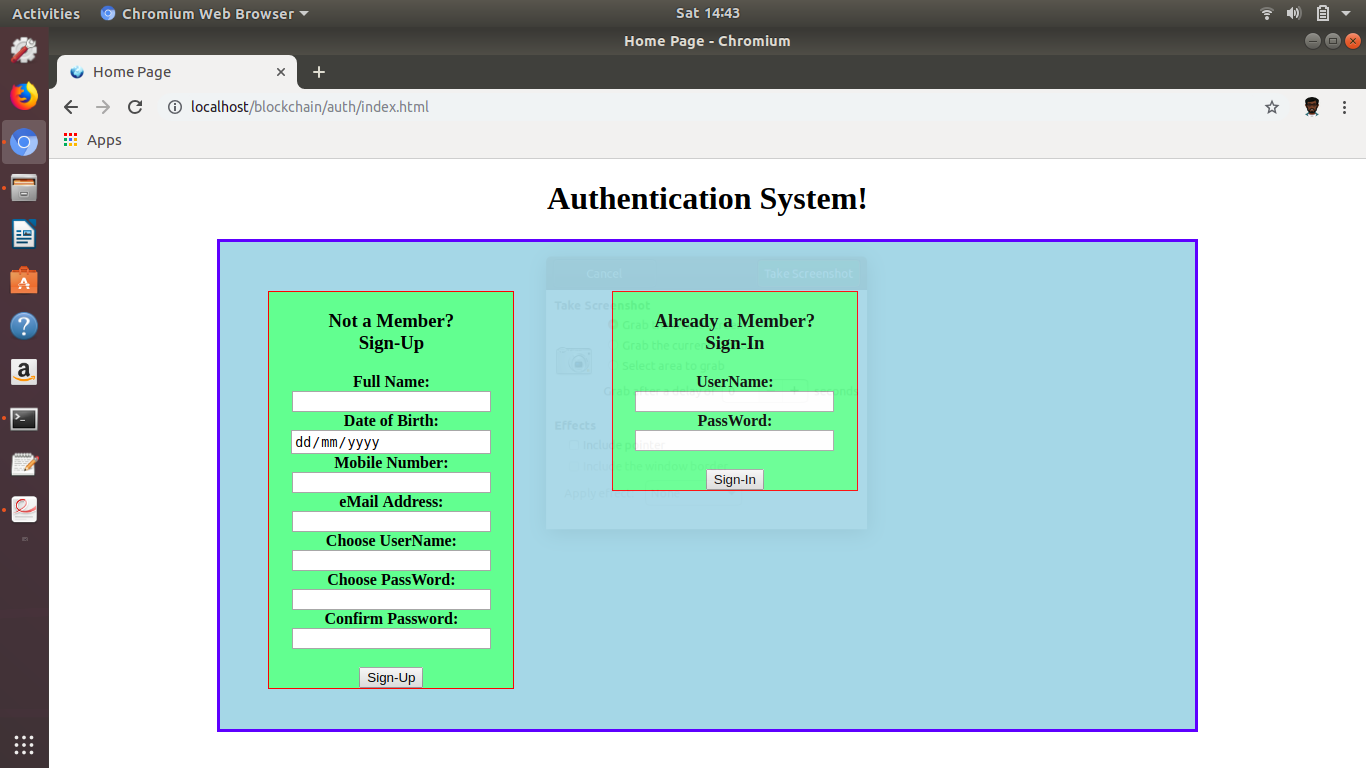
\includegraphics[width=0.75\textwidth]{./img_src/screen0.png}
\end{center}
\caption{Authentication Page}
\label{fig:authorize}
\end{figure}

\begin{figure}
\begin{center}
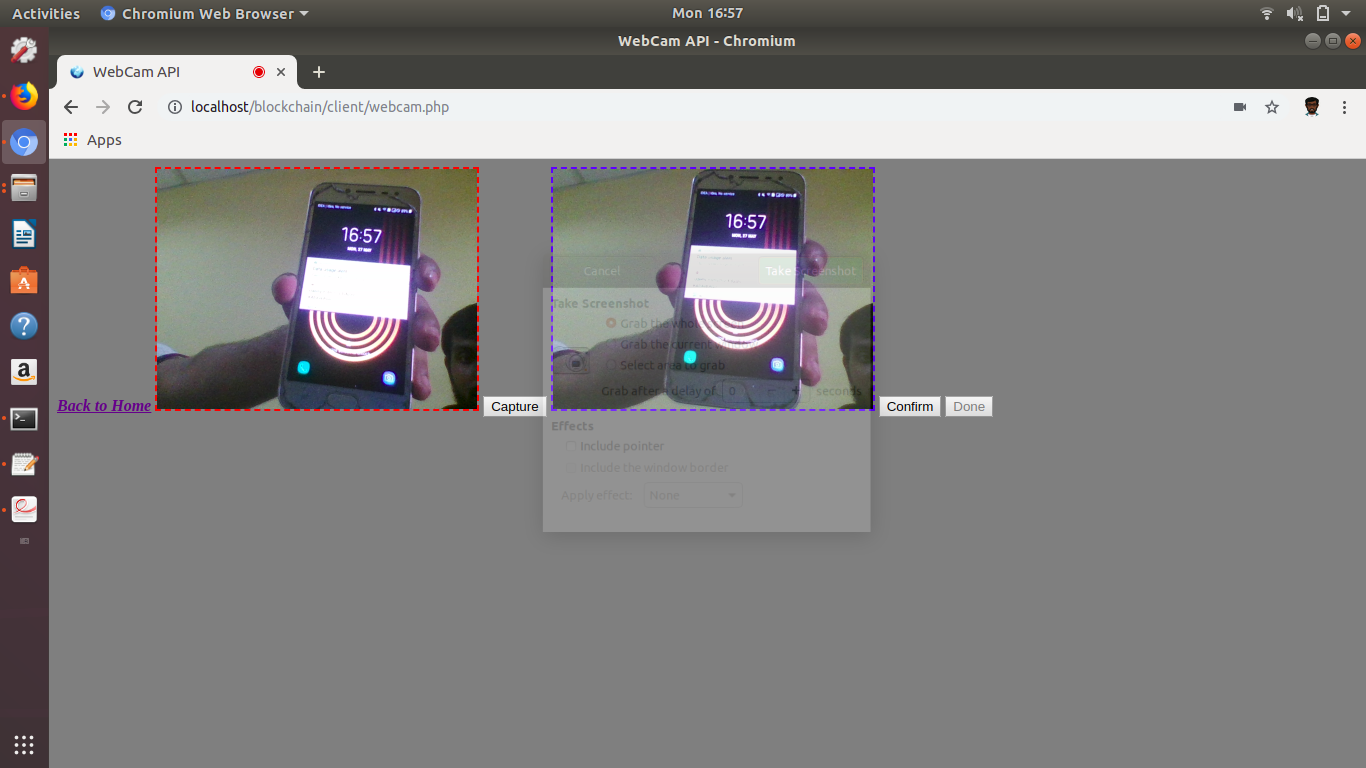
\includegraphics[width=0.75\textwidth]{./img_src/screen1.png}
\end{center}
\caption{Home Page}
\label{fig:homepage}
\end{figure}

\begin{figure}
\begin{center}
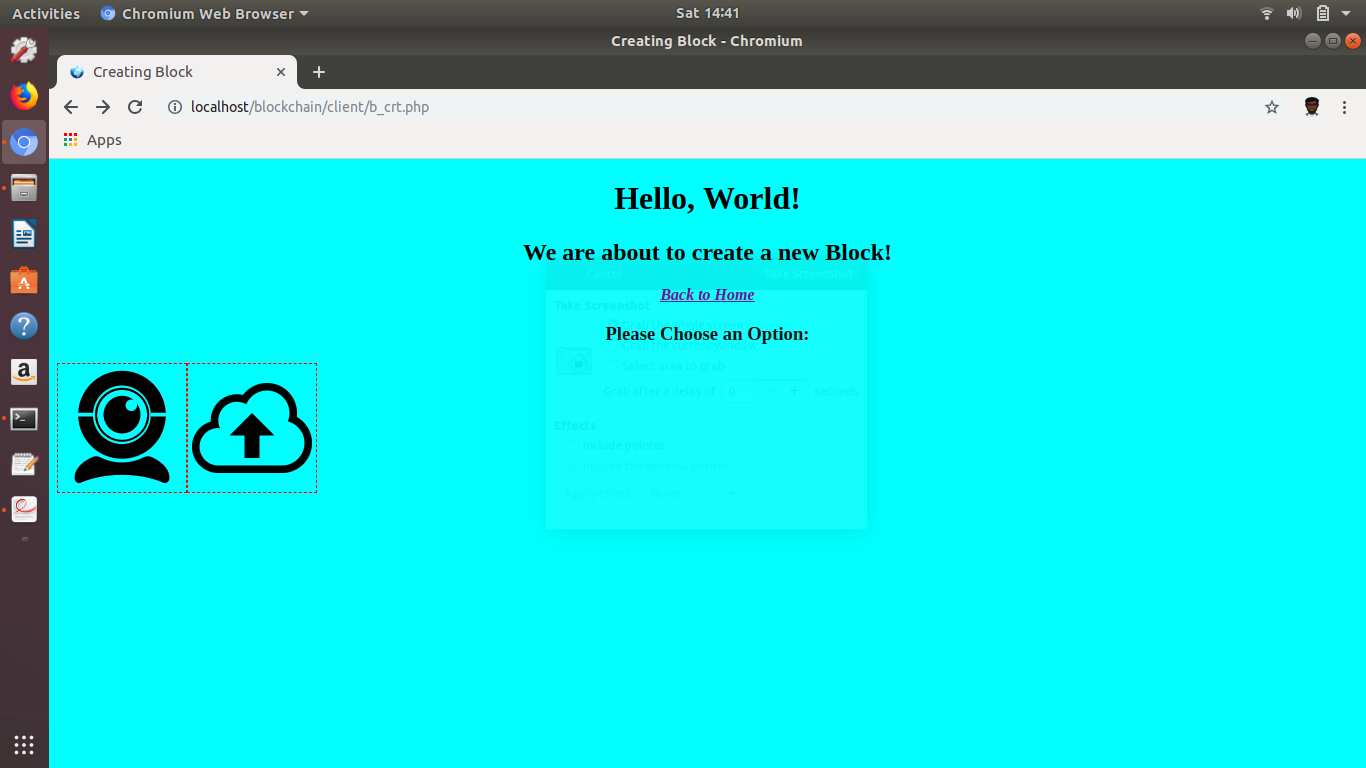
\includegraphics[width=0.75\textwidth]{./img_src/screen2.png}
\end{center}
\caption{Choose How to Insert Image}
\label{fig:img_insert}
\end{figure}

\begin{figure}
\begin{center}
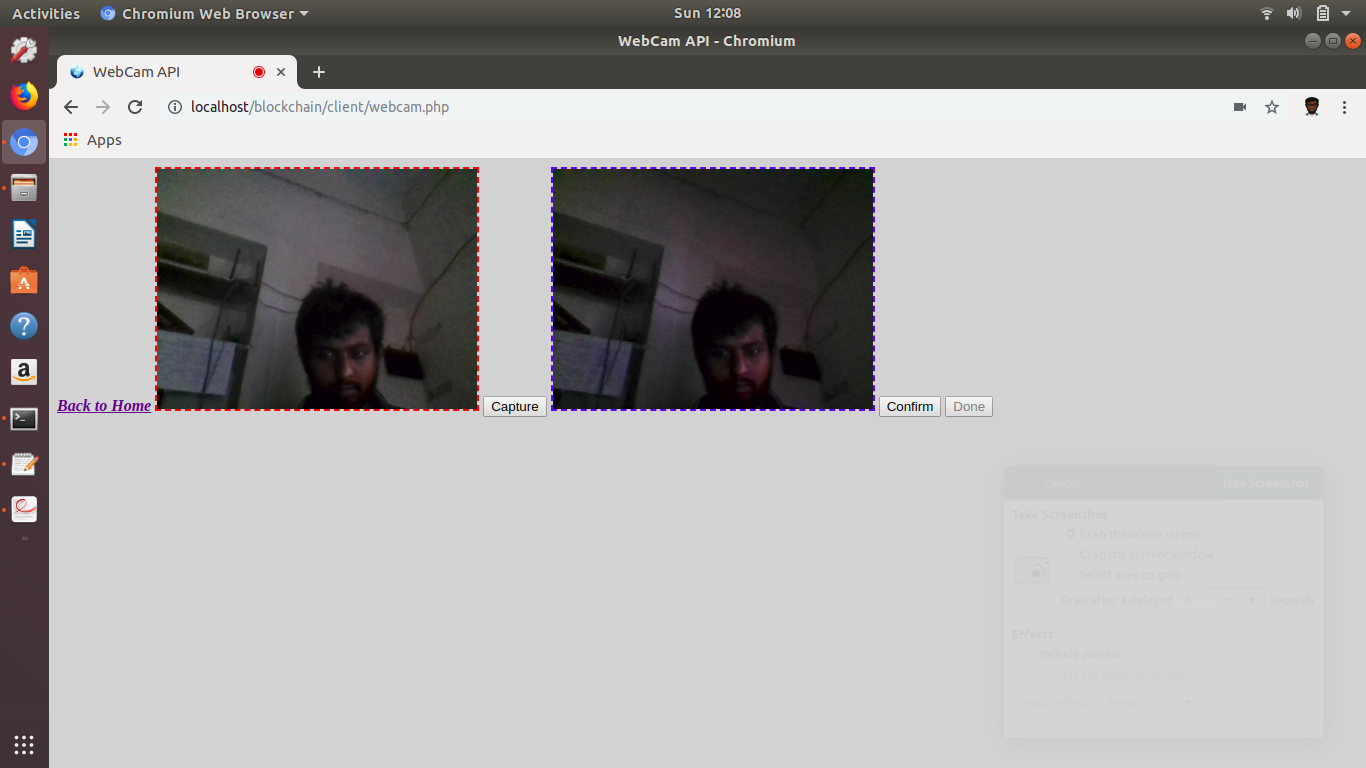
\includegraphics[width=0.75\textwidth]{./img_src/screen3.png}
\end{center}
\caption{WebCam}
\label{fig:img_webcam}
\end{figure}

\begin{figure}
\begin{center}
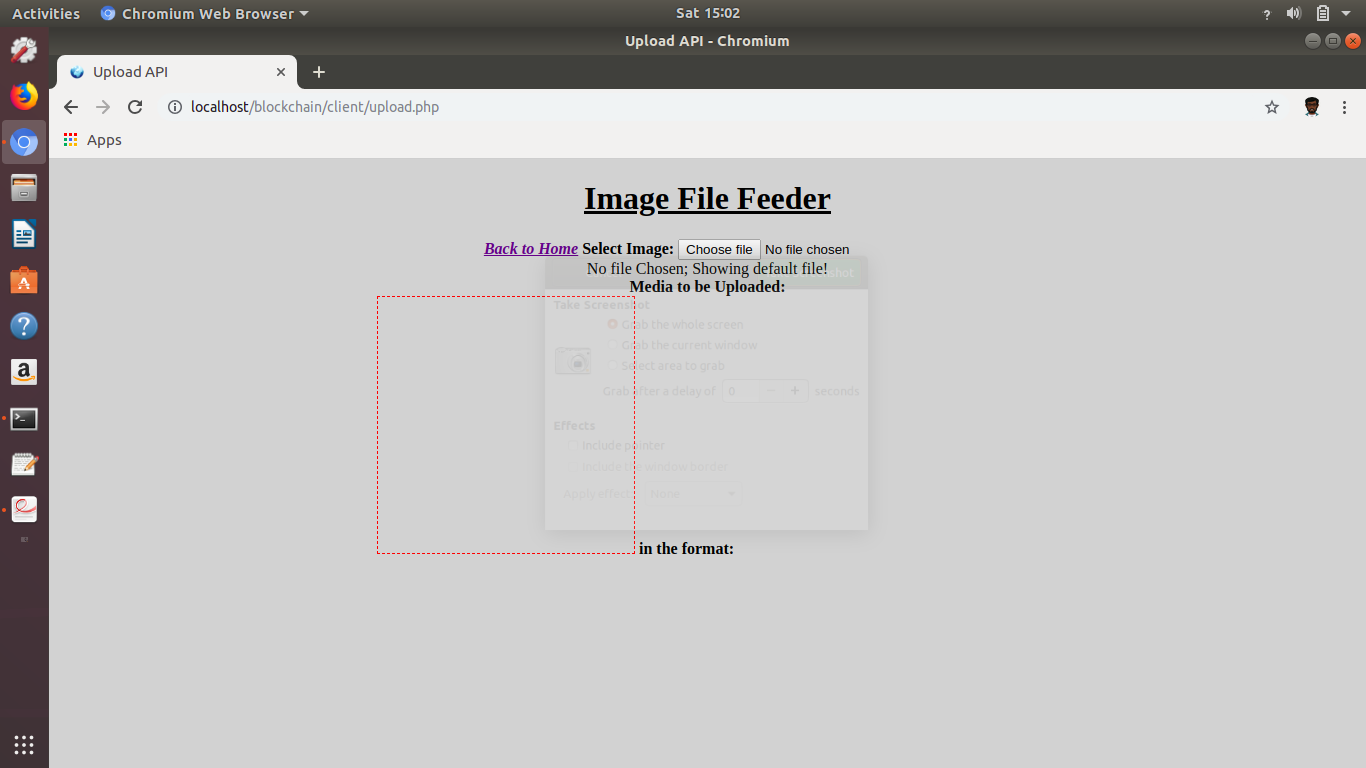
\includegraphics[width=0.75\textwidth]{./img_src/screen4.png}
\end{center}
\caption{Upload}
\label{fig:img_upload}
\end{figure}

\begin{figure}
\begin{center}
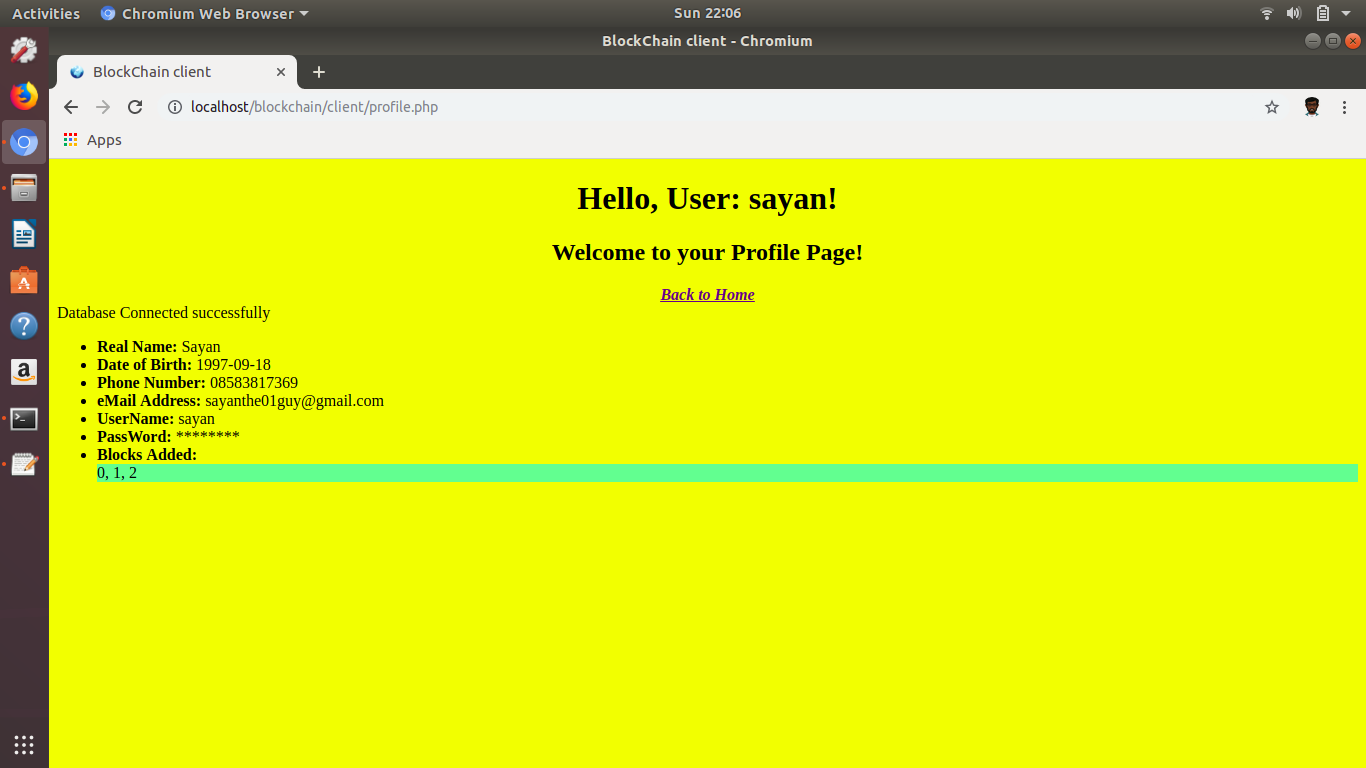
\includegraphics[width=0.75\textwidth]{./img_src/screen5.png}
\end{center}
\caption{Profile}
\label{fig:profile}
\end{figure}

\begin{figure}
\begin{center}
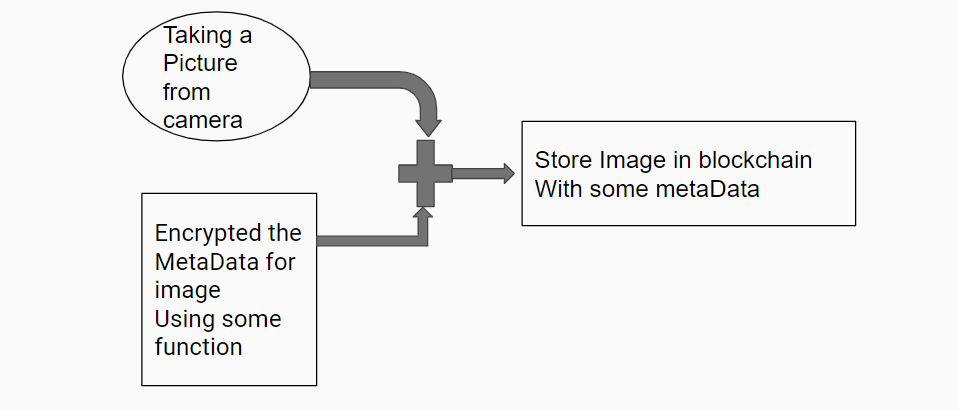
\includegraphics[width=0.75\textwidth]{./img_src/upload.png}
\end{center}
\caption{Image Insertion}
\label{fig:upload}
\end{figure}

\begin{figure}
\begin{center}
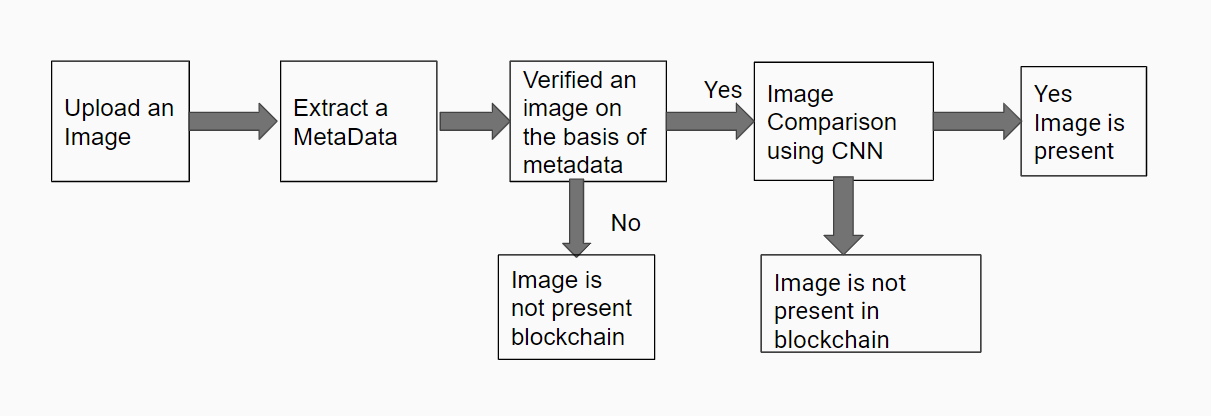
\includegraphics[width=0.75\textwidth]{./img_src/verify.png}
\end{center}
\caption{Image Verification}
\label{fig:verify}
\end{figure}
